\documentclass{article}
\usepackage{graphicx}
\usepackage{amsmath}
\usepackage{pgfplots}
\usepackage{physics}
\usepackage{cancel}
\usepackage{enumitem}
\usepackage{txfonts}

\pgfplotsset{compat=1.18}

\newcommand{\Eth}{E_{\text{th}}}

\usepackage[a4paper, top=1cm, bottom=2cm, left=2cm, right=2cm, includehead, includefoot]{geometry}

\begin{document}

\noindent
Physics 4A - Classical Mechanics \hfill Prof. Roger King

\noindent\rule{\textwidth}{0.4pt}

\begin{center}
    \textbf{\LARGE Homework 10} \\
    \vspace{12pt}
    \large Aaron W. Tarajos \\
    \textit{\today}
\end{center}

\noindent\rule{\textwidth}{0.4pt}

\section*{Problem 1}
A 1.95-kg particle is projected with an initial speed of 4.00 m/s along a surface for which $\mu_k = 0.600$.
Find the distance it travels given that: (a) the surface is horizontal; (b) the particle moves up a 30$^\circ$ incline;
(c) the particle moves down a 30$^\circ$ incline.

\subsection*{Solution}
\subsubsection*{Part a:}
The force of friction is given by
\[
	F_k = \mu_k mg
\]
therefore the work done by friction is given by
\[
	W = \mu_k mg x \cos \theta
\]
the work done by friction is also given by the change in kinetic energy so we have
\begin{align*}
	W &= \Delta k \\
	\mu_k mg x \cos \theta &= K_f - K_i \\
	\mu_k mg x \cos \theta &= 0 - \frac{1}{2}mv^2 \\
	x &= - \frac{v^2}{2 \mu_k g \cos \theta}
\end{align*}
For the given values;
\[
	x = - \frac{4.00^2}{2 \cdot 0.600 \cdot 9.81 \cos(180)} = \boxed{1.359\ \text{m}}
\]

\subsubsection*{Part b:}
Now we need to consider the work done by gravity in addition to the work by done kinetic energy because of the incline;
\begin{align*}
	r mg \sin \theta + r \mu_k mg \cos \theta &= \frac{1}{2}mv^2 \\
	rmg\left(\sin\theta + \ mu_k\cos\theta \right) &= \frac{mv^2}{2} \\
	r &= \frac{v^2}{2g\left(\sin\theta + \mu_k\cos\theta\right)}
\end{align*}
Where $r$ is the magnitude of direction along the incline, then evaluating for the given parameters;
\[
	r = \frac{4.00^2}{(2)(9.81)\left(\sin(30) + (0.600)\cos(30)\right)} = \boxed{0.80\ \text{m}}
\]

\subsubsection*{Part c:}
 The equation changes slightly because gravity is now acting in the same direction as the kinetic energy so we have
\[
	r = \frac{4.00^2}{(2)(9.81)\left(-\sin(30) + (0.600)\cos(30)\right)} = \boxed{41.575\ \text{m}}
\]


\section*{Problem 2}
Use the potential energy function U(x) shown in figure below to sketch the corresponding $F_x$ versus x
graph.

\begin{figure}[ht]
    \centering
    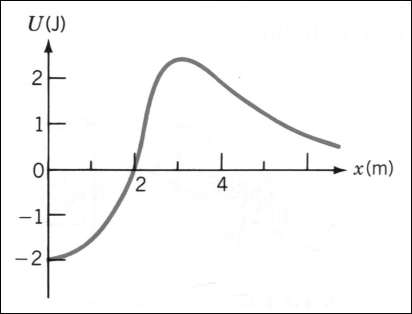
\includegraphics[scale=.5]{drawing-1.png}
\end{figure}

\begin{figure}[ht]
    \centering
    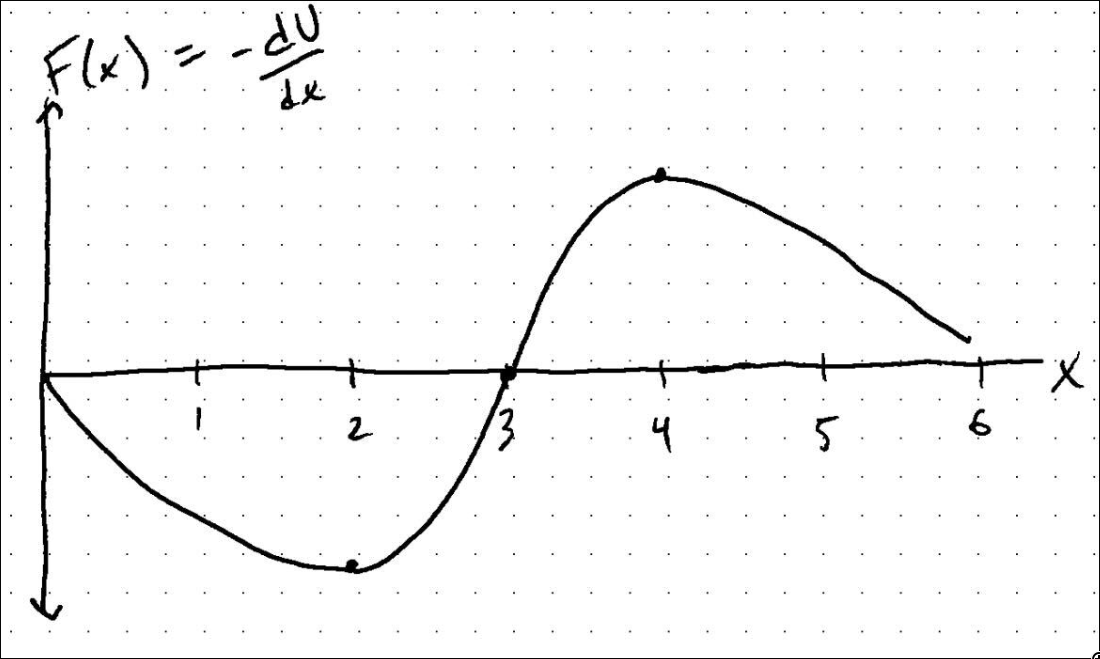
\includegraphics[scale=.20]{graph-1.png}
\end{figure}

\section*{Problem 3}
A 1.75-kg block starts from rest at an initial height of 40.0 cm and slides down a frictionless circular ramp,
as shown in the figure below. It slides for 79.0 cm on the horizontal surface before coming to a stop. What is
the coefficient of kinetic friction? Assume that only the horizontal stretch has friction, and the curved portion
is frictionless.

\begin{figure}[ht]
    \centering
    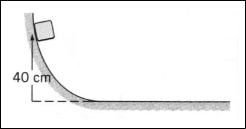
\includegraphics[scale=.5]{drawing-2.png}
\end{figure}

\subsection*{Solution}
The potential energy is of the block at the initial position is given by;
\[
	U_i = mgd
\]
all of which becomes kinetic energy at the bottom of the ramp which is used to solve for velocity.
\begin{align*}
	mgd &= \frac{1}{2} mv^2 \\
	v^2 &= 2gd_1 \\
	v &= \sqrt{2gd_1}
\end{align*}
Then we solve for the friction coefficient using the same method as Problem 1;
\begin{align*}
	W &= \Delta K \\
	F_k \cdot d_2 &= 0 - \frac{1}{2}m \sqrt{2gd_1}^2 \\
	\mu_k mg d_2 \cos \theta &= - \frac{1}{2}m2gd_1 \\
	\mu_k &= -\frac{d_1}{d_2 \cos \theta}
\end{align*}
therefore;

\[
	\mu_k = -\frac{40.0}{79.0 \cos (180)} = \boxed{0.506}
\]

\section*{Problem 4}
The potential energy shared by two atoms separated by a distance r in a diatomic molecule is given by the
Lennard-Jones function ($U_0$ and $r_0$ are constants):

\[
	U(r) = U_0 \left[ \left( \frac{r_0}{r} \right)^{12} - 2 \left( \frac{r_0}{r}\right)^6 \right]
\]
(a) Where is $U(r)=0$ ? (b) Show that the minimum potential energy is $-U_0$ and that it occurs at $r_0$. (c)
Where is $F_r = 0$ ? (d) Sketch $U(r)$.

\subsection*{Solution}
\subsubsection*{Part a:}
\begin{align*}
	0 &= U_0 \left[ \left( \frac{r_0}{r} \right)^{12} - 2 \left( \frac{r_0}{r}\right)^6 \right] \\
	0 &= \left( \frac{r_0}{r} \right)^{12} - 2 \left( \frac{r_0}{r}\right)^6 \\
	\left( \frac{r_0}{r} \right)^{12} &= 2 \left( \frac{r_0}{r}\right)^6 \\
	r_0^{12} &= 2 r_0^6 r^6 \\
	\frac{r_0^6}{2} &= r^6 \\
	r &= \frac{r_0}{\sqrt[6]{2}}
\end{align*}

\subsubsection*{Part b:}
First find the critical points by evaluating $U^\prime(r) = 0$;
\begin{align*}
	U^\prime (r) &= \frac{dU}{dr} \left[ U_0\left( \frac{r_0}{r} \right)^{12} - 2 U_0\left( \frac{r_0}{r}\right)^6 \right] \\
		     &= \frac{12U_{0} r_{0}^{6}}{r^{7}} - \frac{12U_{0} r_{0}^{12}}{r^{13}} \\
	\frac{12U_{0} r_{0}^{12}}{r^{13}} &= \frac{12U_{0} r_{0}^{6}}{r^{7}} \\
	\frac{r_0^{12}}{r^{13}} &= \frac{r_0^6}{r^7} \\
	r_0^6 &= r^6 \\
	r &= r_0
\end{align*}
Now we evaluate $U(r)$ at $r = r_0$;
\begin{align*}
	U(r) = U_0 \left[ \left( \frac{r_0}{r_0} \right)^{12} - 2 \left( \frac{r_0}{r_0}\right)^6 \right] \\
	&= U_0 \left[ 1^12 - 2 \cdot 1^6 \right] \\
	&= U_0 (-1) \\
	&= -U_0
\end{align*}
Because function is decreasing to the left of $r_0$ and increasing to the right of $r_0$ it must be a local minimum and the given potential energy is $U(r_0) = -U_0$. $\blacksquare$

\subsubsection*{Part c:}
$F_r = 0$ when $-\frac{dU}{dr} = 0$. We already solved for $\frac{dU}{dr} = 0$ and found that it is at $r = r_0$. Therefore $F_r = 0$ when $r = r_0$.

\subsubsection*{Part d:}
\begin{figure}[ht]
    \centering
    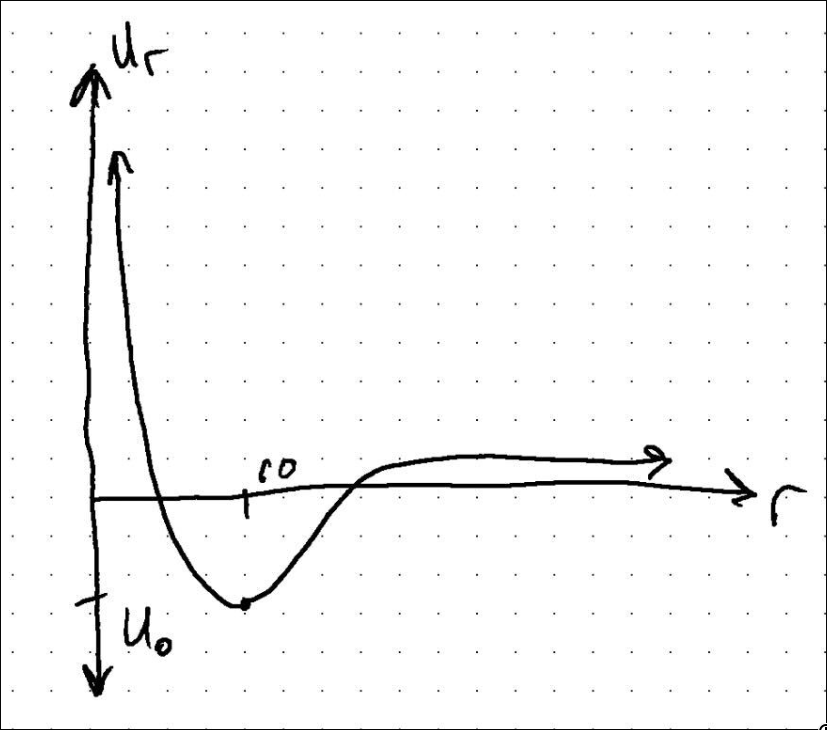
\includegraphics[scale=.20]{graph-2.png}
\end{figure}

\section*{Problem 5}
In the figure below, a 3.50 kg block is accelerated from rest by a compressed spring of spring constant 640
N/m. The block leaves the spring at the spring’s relaxed length and then travels over a horizontal floor with a
coefficient of kinetic friction $\mu_k$ = 0.25. The frictional force stops the block in distance $D$ = 7.80 m. What are
(a) the increase in the thermal energy of the block–floor system, (b) the maximum kinetic energy of the block,
and (c) the original compression distance of the spring?

\begin{figure}[ht]
    \centering
    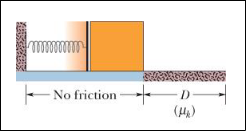
\includegraphics[scale=.5]{drawing-3.png}
\end{figure}

\subsection*{Solution}
\subsubsection*{Part a:}
The initial thermal energy, $E_{\text{th}}$ is given by
\begin{align*}
	\Eth &= F_k \cdot d \\
	     &= \mu_k mg \cdot d \\
	     &= (0.25)(3.50)(9.81)(7.80) \\
	     &= \boxed{66.953\ \text{J}}
\end{align*}

\subsubsection*{Part b:}
All of the kinetic energy is turned into $\Eth$ because the block has zero $K_f$ when it stops. Therefore;
\[
	K_\text{max} = \Eth = \boxed{66.953\ \text{J}}
\]

\subsubsection*{Part c:}
The spring compression is solve for by solving for $x$ in the potential energy equation, and because the potential energy generated by the spring is equal to the maximum kinetic energy, we have
\begin{align*}
	\frac{1}{2}kx^2 &= K_\text{max} \\
	x &= \sqrt{\frac{2 K_\text{max}}{k}} \\
	x &= \sqrt{\frac{2 \mu_k mg \cdot d}{k}} \\
	x &= \sqrt{\frac{2 \cdot 0.25 \cdot 3.50 \cdot 9.81 \cdot 7.80}{640}} \\
	  &= \boxed{0.457 \ \text{m}}
\end{align*}



\section*{Problem 6}
The masses and positions of three particles in the $xy$ plane are as follows: 2.05 kg at (-2.00, 3.00) m; 3.00 kg
at (-3.00, 4.00) m, and; and 5.00 kg at (3.00, -1.00) m. What is the position of the CM?

\subsection*{Solution}
The center of mass in the $x$ direction is
\[
	x = \frac{m_1 x_1 + m_2 x_2 + m_3 x_3}{m_1 + m_2 + m_3} = \frac{(2.05)(-2.00)+(3.00)(-3.00)+(5.00)(3.00)}{2.50 + 3.00 + 5.00} = 0.181\ \vu i
\]
similarly for $y$;
\[
	y = \frac{m_1 y_1 + m_2 y_2 + m_3 y_3}{m_1 + m_2 + m_3} = \frac{(2.05)(3.00) + (3.00)(4.00) + (5.00)(-1.00)}{2.50 + 3.00 + 5.00} = 1.252\ \vu j
\]
Therefore the center of mass is;
\[
	\boxed{ CM = 0.181\ \vu i + 1.252\ \vu j \ \text{m}}
\]

\section*{Problem 7}
A block of mass $m_1$ = 2.00 kg has velocity $\va{u}_1 = 5.00 \vu{i} - 3.00 \vu{j} + 4.00 \vu{k}$ m/s and another block of mass
$m_2$ = 6.00 kg has a velocity $\va{u}_2 = -3.00 \vu{i} + 2.00 \vu{j} - 1.00 \vu{k}$ m/s. (a) What is the velocity of the CM? (b)
What is the total momentum of the system of two blocks?

\subsection*{Solution}
\subsubsection*{Part a:}
The velocity of the CM is evaluated using the same method as position so we have;
\begin{align*}
	v_x &= \frac{(2.00)(5.00) + (6.00)(-3.00)}{8.00} = -1\ \vu i \\
	v_y &= \frac{(2.00)(-3.00) + (6.00)(2.00)}{8.00} = 0.75\ \vu j \\
	v_z &= \frac{(2.00)(4.00) + (6.00)(-1.00)}{8.00} = 0.25\ \vu k \\
	\va v_{CM} &= \boxed{-1 \vu i + 0.75\ \vu j + 0.25\ \vu k \ \text{m}/\text{s}}
\end{align*}

\subsubsection*{Part b:}
The momentum is given by
\[
	\va p = m \va v
\]
and the total momentum is the sum of the individual object momentum given by the numerator of $\va v_{CM}$;
\[
	\va p_{\text{total}} = \boxed{-8.00\ \vu i + 6.00\ \vu j + 2.00\ \vu k \ \text{kg}\cdot\text{m}/\text{s}}
\]

\section*{Problem 8}
Use integration to locate the CM of the triangular plate of base $b$ and height $h$ shown in the figure below.
The plate has a uniform areal mass density $\sigma$ (mass per unit area).

\begin{figure}[ht]
    \centering
    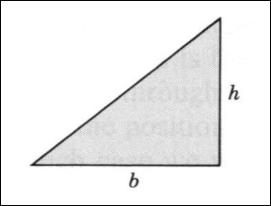
\includegraphics[scale=.5]{drawing-4.png}
\end{figure}

\subsection*{Solution}
The center of mass along the $x$ axis is given by;
\begin{align*}
	x_{CM} &= \frac{1}{A} \int_a^b x f(x)\ dx \\
	&= \frac{2}{bh} \int_0^b x \left(\frac{h}{b}x\right)\ dx \\
	&= \frac{2}{b^2} \int_0^b x^2 \ dx \\
	&= \frac{2x^3}{3b^2} \biggr\rvert_0^b \\
	&= \frac{2b}{3}
\end{align*}

Then the center of mass along the $y$ axis is given by;
\begin{align*}
	y_{CM} &= \frac{1}{A} \int_a^b \frac{1}{2} \left[ f(x) \right]^2\ dx \\
	       &= \frac{2}{bh} \int_0^b \frac{1}{2} \left[ \frac{h^2x^2}{b^2} \right] \ dx \\
	       &= \frac{h}{b^3} \int_0^b x^2 \ dx \\
	       &= \frac{hx^3}{3b^3} \biggr\rvert_0^b \\
	       &= \frac{h}{3}
\end{align*}
Giving us the center of mass;

\[
	\left( x_{CM}, y_{CM}\right) = \boxed{\left( \frac{2b}{3}, \frac{h}{3} \right)}
\]


\end{document}
